\chapter{Entorno y herramientas}
\label{cap:entorno}
En este capítulo se presentaran y describirán las herramientas hardware y software que se han usado para el desarrollo del proyecto. En primer lugar se presentará el robot sobre el que hemos trabajado, el robot kobuki. En segundo lugar se presentará el \textit{framework} sobre el que hemos construido el algoritmo, ROS , y por ultimo se describirán las herramientas de dicho framework que han resultado esenciales para la realización del proyecto.


\section{Robot Kobuki}
\label{cap:robot}
El robot kobuki o Turtlebot es un robot \textit{lowcost} que cuenta con un software de código abierto. Su estructura principal es una base móvil de forma circular y una serie de baldas y barras metálicas para adaptar su configuración física a nuestras necesidades. Cuenta con una integración total con ROS, el framework que se usará para el proyecto, y además es el robot usado por la mayoría de alumnos de la universidad para cursar la asignatura de robótica.
\begin{figure} [H]
  \begin{center}
    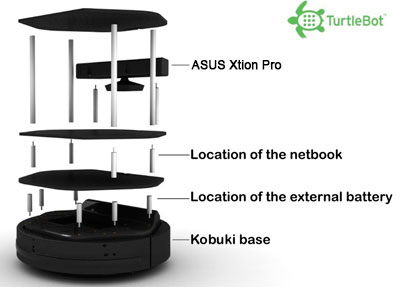
\includegraphics[width=7.5cm]{img/cap3/kobuki}
  \end{center}
  \caption{Robot kobuki.}
  \label{fig:kobuki}
\end{figure}

Cuenta con una autonomía de unas 5 horas y es capaz de cargar 5 kg de peso. Además cuenta con multitud de puertos que nos facilitarán la alimentación de los nuevos sensores que queramos incluirle. 

\begin{figure} [H]
  \begin{center}
    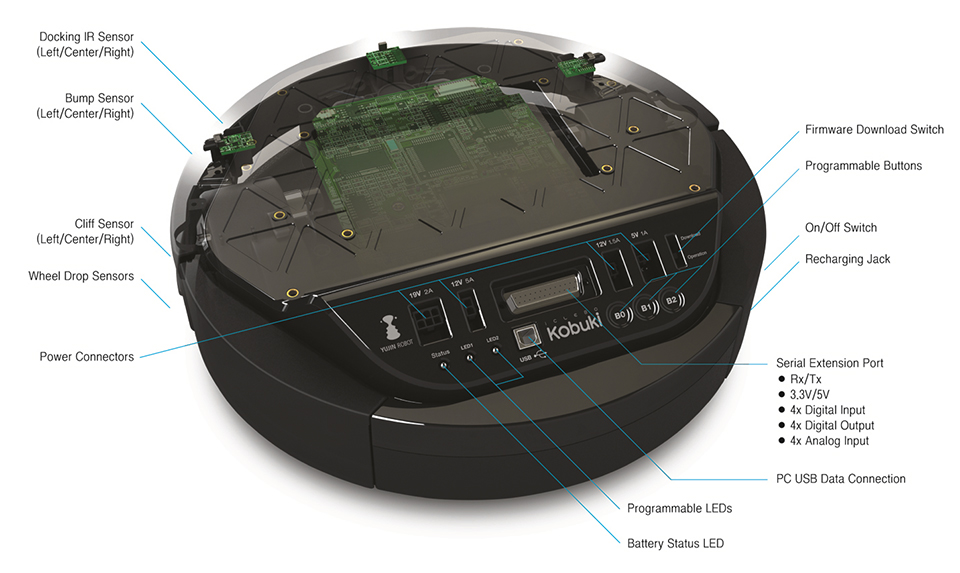
\includegraphics[width=12cm]{img/cap3/kobukispec}
  \end{center}
  \caption{Especificaciones robot kobuki.}
  \label{fig:espckobuki}
\end{figure}

\section{ROS}
\label{cap:ros}
ROS, cuyas siglas significan \textit{Robot Operating System},es un framework muy flexible para al creación de software para robots. Cuenta con una amplia colección de herramientas y librerías que nos simplifican la generación de comportamientos, tanto simples como complejos, para una gran variedad de plataformas. Este framework se ha convertido en el estándar en el ámbito de la programación de software para robots por su gran versatilidad y su gran robustez y por proporcionarnos abstracción del hardware, control sobre los dispositivos de bajo nivel, paso de mensajes entre procesos y mantenimiento de paquetes gracias a sus repositorios.

La idea fundamental de ROS es la utilización de \textit{topics} como modelo de comunicación entre procesos, que en ROS se les llama nodos. En estos \textit{topics} los nodos publican los mensajes o la información que desean comunicar y otros nodos estarán subscritos a esos \textit{topics} para leer dicha información. Dichos nodos están totalmente perfectamente distribuidos, lo que permite el procesamiento distribuido en múltiples núcleos, multiprocesamiento, GPUs y clústeres. Otro modelo de comunicación usado en ROS, aunque no es el principal, es el del uso de \textit{actionlib}\footnotemark. Esta herramienta puede ser descrita como la petición de la realización de una acción a un nodo y la espera de la finalización de esta.

ROS incluye paquetes que pueden cubrir diferentes áreas como: 
\begin{itemize}
\item Percepción.
\item Identificación de Objetos.
\item Segmentación y reconocimiento.
\item Reconocimiento facial.
\item Reconocimiento de gestos.
\item Seguimiento de objetos.
\item Comprensión de movimiento.
\item Estructura de movimientos (SFM).
\item Visión estéreo: percepción de profundidad mediante el uso de dos cámaras.
\item Visión 3D mediante el uso de cámaras RGBD.
\item Movimientos.
\item Robots móviles.
\item Control.
\item Planificación.
\item Agarre de objetos.
\end{itemize}
\footnotetext{http://wiki.ros.org/actionlib}

ROS también cuenta con una integración perfecta con visualizadores de información, como puede ser \textit{Rviz}, o con el simulador \textit{Gazebo}. Esto resulta especialmente útil en un entorno de desarrollo robótico, ya que tanto los robots como los sensores que utilizamos habitualmente tienen un coste alto y cuanto más los cuidemos y más desarrollemos sobre un simulador más alargaremos su vida útil. Esto no significa que tengamos que desarrollar el 100\% de nuestros experimentos sobre el simulador, ya que todo algoritmo robótico llevado al robot real difiere bastante del algoritmo desarrollado para el simulador. En un entorno real nos encontraremos con muchos inconvenientes y problemas que el simulador nos da resueltos y tendremos que preparar nuestro algoritmo para que sea robusto frente a estos problemas.

En la figura \ref{fig:modelocomunicacion} vemos un esquema de una aplicación y su modelo de comunicación. La aplicación en concreto es \textit{move\_base},de la que hablaremos un poco más adelante y que está representada con el cuadro negro central. Dentro de este cuadro tenemos los distintos nodos que componen la aplicación. En las flechas que entran a la aplicación tenemos los \textit{topics} a los que está subscrito la aplicación y en las flechas de salida se representan los \textit{topics} en los que la aplicación publica. En estas flechas también está representado el tipo de mensaje que se publica en estos \textit{topics}. Estos mensajes son estándar de ROS, están creados y se pueden componer fácilmente en nuestros nodos, por lo que resulta la mejor manera de comunicar nuestros nodos. También podemos crear nuestros mensajes propios, pero esto rompe un poco el estándar. 

\begin{figure} [H]
  \begin{center}
    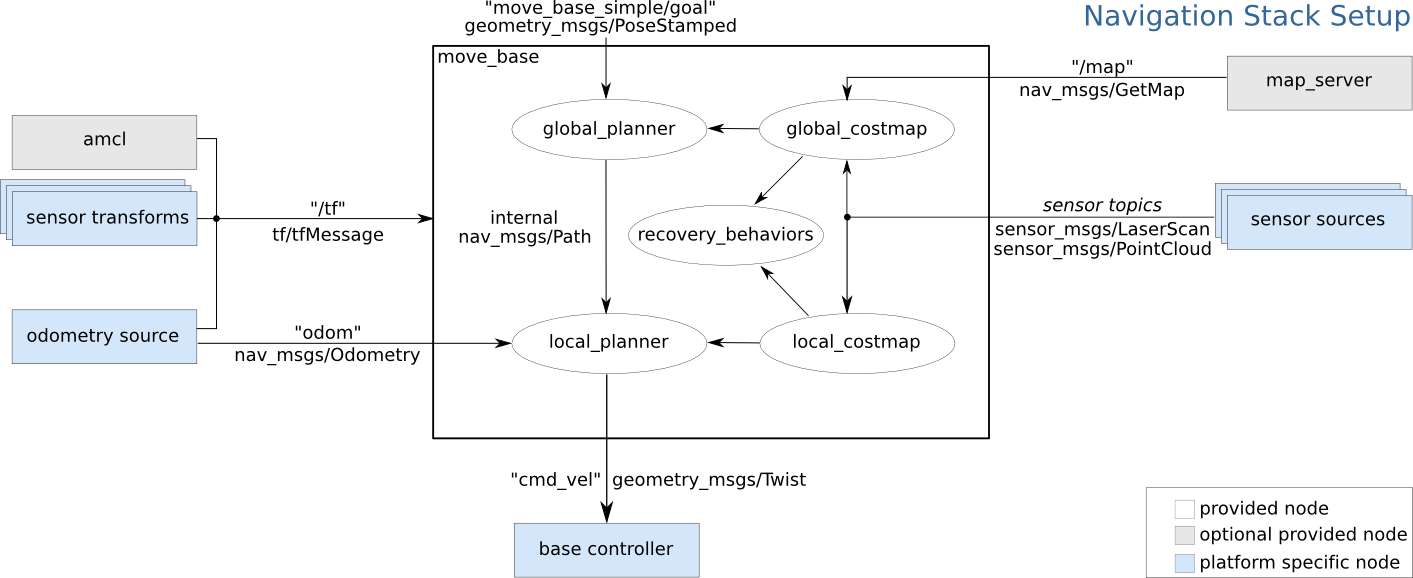
\includegraphics[width=16cm]{img/cap3/navigationstack}
  \end{center}
  \caption{Representación del modelo de comunicación de ROS.}
  \label{fig:modelocomunicacion}
\end{figure}

Ahora hablaremos un poco más en profundidad de la herramienta que está representada por el topic a la izquierda de la aplicación, \textit{tf}

\subsubsection{tf}
\label{subsubsec:tf}
Cualquier robot está compuesto por multitud de piezas móviles, como puede ser la propia base del robot o la pinza de un brazo robótico. Cada una de estas piezas se pueden representar con un \textit{frame}. Ademas existen también otros \textit{frames} que pueden interesarnos, como puede ser el \textit{frame} de world o el \textit{frame} de map.
\begin{figure} [hbtp]
  \begin{center}
    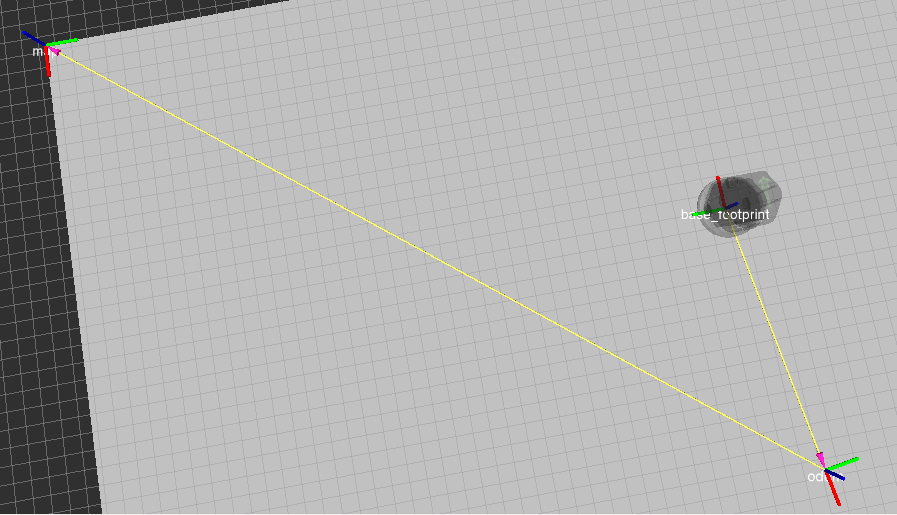
\includegraphics[width=12cm]{img/cap3/frames}
  \end{center}
  \caption{A la izquierda el frame map y a la derecha los frames de odom y base\_footprint}
  \label{fig:frames}
\end{figure}

Usamos las \textit{tf} para poder representar información relativa a uno de estos frames. Esto puede sernos de utilidad, por ejemplo, si queremos conocer la posición de un objeto que hemos cogido con nuestra pinza respecto a la base de nuestro robot, o cual es la posición relativa de un objeto que estamos percibiendo con el láser respecto a nosotros o respecto al mapa.

Cuando trabajamos con mapas es importante que todo lo que se representa en él sea respecto al frame \textit{map}. De este modo nuestro mapa puede ser usado por otros nodos, como el nodo de navegación, o por otro robot situado en el escenario representado en el mapa.


\section{Software en ROS para el mapeado, localización y navegación}
\label{cap:softwarederos}
En esta sección se describirá el funcionamiento de los diferentes paquetes que ROS nos proporciona y que resultan esenciales para la creación de mapas, la localización y la navegación por distintos entornos.

\subsection{Costmap\_2D}
\label{sec:costmap2d}
Un \textit{costmap} es una estructura de datos ofrecida por ROS y compuesta por un grid de ocupación y los metadatos de este grid. Cada celda del grid toma valores entre 0 y 255, donde 0 corresponde a una celda vacía, los valores entre 1 y 254 representan la probabilidad de que una celda está ocupada y el valor 255 se reserva para el total desconocimiento sobre el estado de una celda. Cada valor se asocia con un nivel de gris, como se puede ver en la imagen.
\begin{figure} [H]
  \begin{center}
    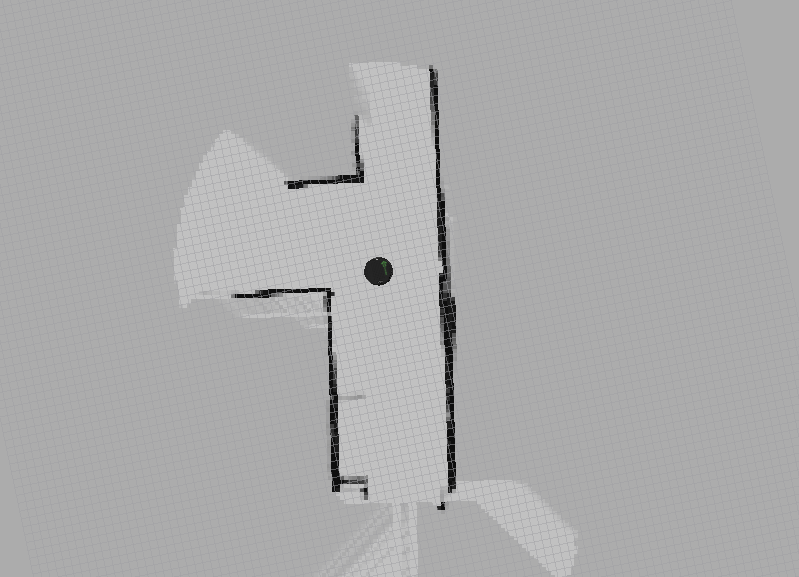
\includegraphics[width=7.5cm]{img/cap3/costmap-ejemplo}
  \end{center}
  \caption{Ejemplo visual de un costmap.}
  \label{fig:costmap-ejemplo}
\end{figure}\

Para poder representar la ocupación de un objeto en un \textit{costmap} es necesario hacer uso de las transformadas entre frames que nos ofrece ROS.

\subsection{Map\_server}
\label{sec:mapserver}
El nodo \textit{map\_server} es un nodo muy simple y muy útil. Se encarga de cargar un mapa en formato \textit{.pgm} de un fichero y publicarlo en un topic para que nodos como \textit{amcl} o \textit{move\_base} se alimenten de él.

\subsection{Map\_saver}
\label{sec:mapsaver}
El nodo \textit{map\_saver} se encarga de guardar en un fichero \textit{.pgm} el mapa que se está publicando en un topic.

\subsection{AMCL}
\label{sec:amcl}
\textit{AMCL}\footnote{http://wiki.ros.org/amcl} es un paquete de localización que implementa un algoritmo de Monte Carlo, el cual usa un filtro de partículas para localizar al robot sobre un mapa que previamente le proporcionamos.
\subsubsection{Filtro de partículas}

El algoritmo del filtro de partículas se divide en 4 etapas: Inicialización, actualización, estimación y predicción. 

\begin{enumerate}
\item Inicialización: En la etapa de inicialización se ``lanzan'' una serie de partículas cercanas a la posición inicial del robot. Estas partículas ademas de una posición en el espacio también tendrán una dirección. Podemos ver un ejemplo gráfico en la imagen \ref{fig:initamcl}. Vemos como se han generado muchas partículas alrededor del robot y que cada una tiene una dirección más o menos acertada con la dirección del robot.
\item Actualización: En este punto del algoritmo se compara la percepción del láser del robot en el punto en el que se encuentra con la percepción que tendría si tuviera la posición y la dirección de cada una de las partículas que generamos. Cuanto más acertada sea la suposición anterior, más valor se le da a esa partícula. Así nos encontraremos que las partículas que están más cercanas a la posición del robot cobran más valor y las que están más lejos y con una dirección totalmente errónea tienen menos valor.
\item Estimación: En esta fase nos quedamos con las partículas que más valor tenían para volver a lanzarlas en la siguiente fase del algoritmo.
\item Predicción: En esta última fase lanzamos las partículas de nuevo con el valor que tenían y su posición, añadiéndole un pequeño ruido.
En este punto del algoritmo también se corrige la posición del robot a la posición de la partícula con más valor.
Una vez completado el algoritmo se vuelve a la fase de Actualización y se repite hasta que el robot esté perfectamente localizado en el 
mapa.
\end{enumerate}

\begin{figure}[hbtp]
  \begin{center}
    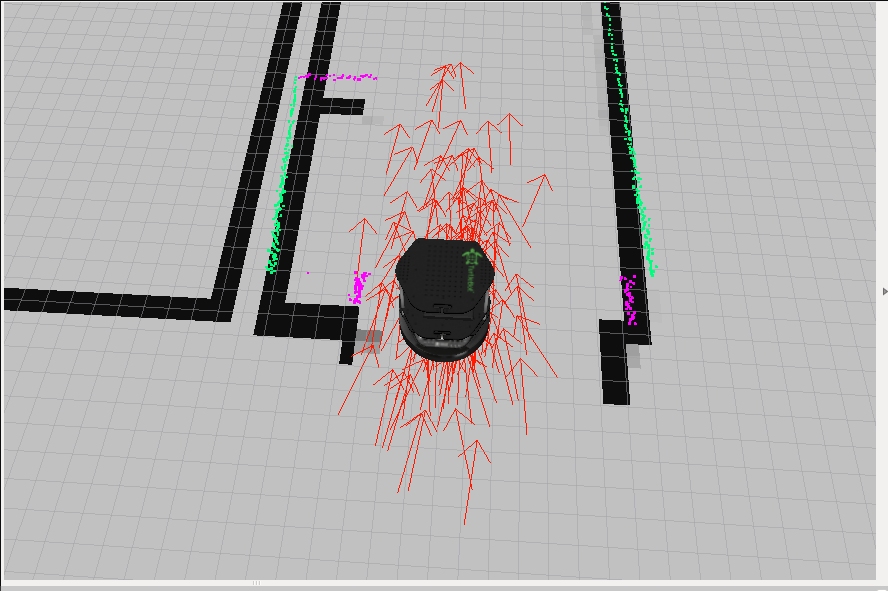
\includegraphics[width=10cm,height=7cm]{img/cap3/initamcl}
  \end{center}
  \caption{Inicialización del filtro de partículas}
  \label{fig:initamcl}
\end{figure}


\begin{figure}[hbtp]
  \begin{center}
    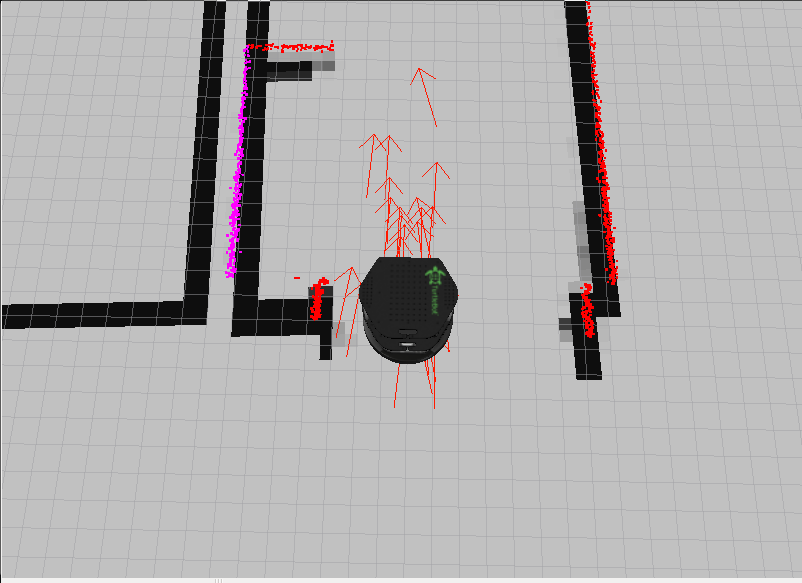
\includegraphics[width=10cm,height=7cm]{img/cap3/actamcl}
  \end{center}
  \caption{El robot se vá acercando a la posición ideal}
  \label{fig:actamcl}
\end{figure}

Observamos como la linea color de la parte derecha de la imagen \ref{fig:actamcl}, correspondiente a las muestras tomadas con el láser, está más cerca de la linea del mapa que en la imagen \ref{fig:initamcl} que se aprecia que no está alineada. Esto es fruto de la corrección que se va haciendo de la posición. También observamos que hay menos partículas, esto es fruto de la convergencia hacia la posición correcta.

\begin{figure}[hbtp]
  \begin{center}
    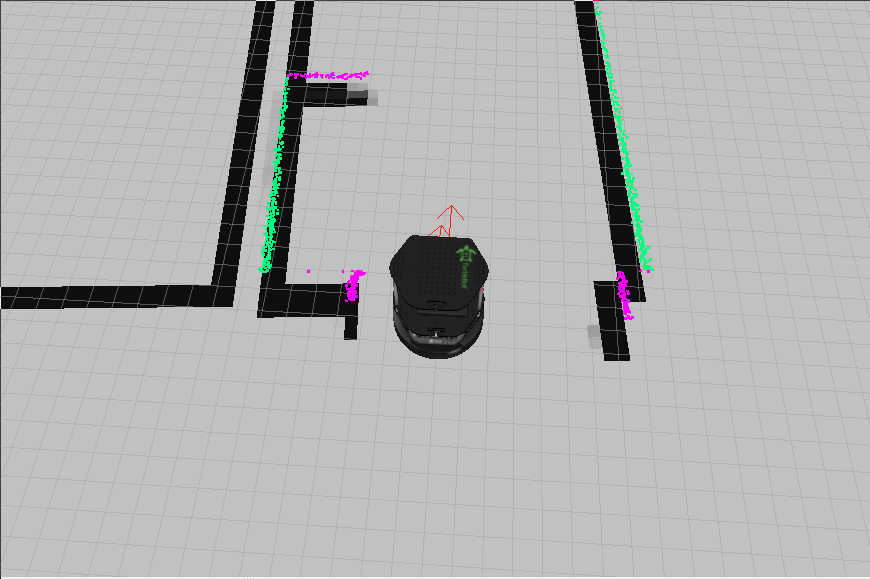
\includegraphics[width=10cm,height=7cm]{img/cap3/finamcl}
  \end{center}
  \caption{El robot se encuentra totalmente localizado.}
  \label{fig:finamcl}
\end{figure}

En la imagen \ref{fig:finamcl} vemos como el número de partículas se ha reducido mucho, ya que se ha llegado a casi una estimación de la posición del robot muy cerca de la posición real. Vemos también que las lineas de color correspondientes a las muestras del láser están alineadas con el mapa.

()()) Habrá que ponerlo en otro sitio

Para el uso del paquete \textit{amcl} en nuestro algoritmo fue necesaria la realización de una pequeña modificación. Esta modificación se refiere a que el paquete por defecto solo usa un mapa y lo obtiene al principio de la ejecución del algoritmo. Si le llegaba un nuevo mapa reiniciaba por completo el algoritmo. Esto nos generaba un problema, ya que en el algoritmo propuesto se publica un mapa por cada iteración y el paquete por defecto se reiniciaba constantemente. El efecto que producía es que el robot siempre se encontraba en la posición inicial y aunque lo moviéramos siempre ocupaba la misma posición en el mapa. En nuestro \textit{amcl} modificado se usa el mapa que se obtiene en cada iteración y sobre el se calcula la posición del robot, sin reiniciar en ningún momento el algoritmo.

())()

\subsection{Move\_base}
\label{sec:movebase}
El paquete principal para la navegación es el paquete \textit{move\_base}\footnotemark. Este paquete es el encargado de, proporcionándole un punto de meta y un mapa sobre el que navegar, calcular el plan necesario para llegar hasta dicho punto y ejecutar dicho plan para que el robot alcance su destino. \textit{Move\_base} cuenta nodos que calculan y ejecutan la ruta, \textit{global planner} y \textit{local planner}. El \textit{global planner} se encarga de planificar la ruta teniendo en cuenta el mapa que obtiene del servidor de mapas. Este nodo se asegurará de que la ruta no atraviesa ningún objeto y que la ruta calculada es la mejor para llegar al destino. Para ello creará un nuevo mapa, partiendo del mapa que le proporcionamos, en el que todas las paredes y los objetos están inflados una distancia igual al radio del robot. Además calculará una nueva ruta si el robot se parara a causa de un objeto o si en medio del camino se da cuenta que la ruta no puede llevarse a cabo.
\begin{figure}[H]
  \begin{center}
    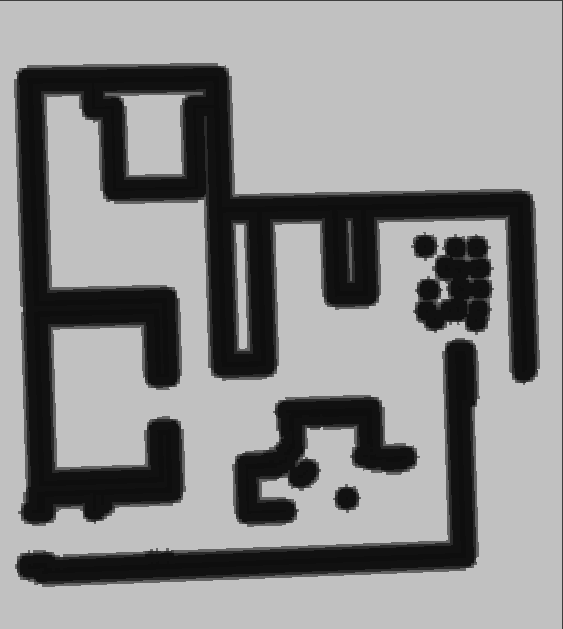
\includegraphics[width=7cm,height=7cm]{img/cap3/movebase}
  \end{center}
  \caption{Mapa de navegación usado por move\_base.}
  \label{fig:movebasemap}
\end{figure}



El \textit{local planner} se encarga de ejecutar el plan calculado por el \textit{global planner}, así como de esquivar objetos que no están en el mapa y de navegar de una forma segura, sin chocar con las paredes o los muebles del escenario.
\footnotetext{http://wiki.ros.org/move\_base?distro=indigo}

\subsection{gmapping}
\label{sec:gmapping}
Este paquete nos proporciona un algoritmo de SLAM, Simultaneous Localization and Mapping, que nos construye un mapa del escenario en el que se encuentre el robot sin pasarle ningún mapa previo del lugar y ademas se localiza en ese mapa a la vez que lo construye. Este paquete hace uso del sensor láser para realizar la construcción del mapa.